\documentclass[12pt]{article}
\usepackage[spanish, english, es-tabla]{babel}
\usepackage[utf8]{inputenc}
\usepackage[left = 2cm, right = 2cm, bottom = 2cm, top = 3cm]{geometry}
\usepackage{amsmath, amssymb}
\usepackage{graphicx}
\usepackage{hyperref}
\usepackage{listings}
\usepackage{courier}

\usepackage[dvipsnames]{xcolor}

\renewcommand{\lstlistingname}{Código}
\renewcommand{\lstlistlistingname}{Listado de códigos}

% https://tex.stackexchange.com/questions/60209/how-to-add-an-extra-level-of-sections-with-headings-below-subsubsection
\newcommand{\subsubsubsection}[1]{\paragraph{#1}\mbox{}\\}
\setcounter{secnumdepth}{4}
\setcounter{tocdepth}{4}

% Configure lstlisting
\definecolor{codegreen}{rgb}{0,0.6,0}
\definecolor{codegray}{rgb}{0.5,0.5,0.5}
\definecolor{codepurple}{rgb}{0.58,0,0.82}
\definecolor{backcolour}{rgb}{0.95,0.95,0.92}

\lstdefinestyle{mystyle}{
	backgroundcolor=\color{backcolour},   
	commentstyle=\color{codegreen},
	keywordstyle=\color{magenta},
	numberstyle=\tiny\color{codegray},
	stringstyle=\color{codepurple},
	basicstyle=\ttfamily\footnotesize,
	breakatwhitespace=false,         
	breaklines=true,                 
	captionpos=t,                    
	keepspaces=true,                 
	numbers=left,                    
	numbersep=5pt,                  
	showspaces=false,                
	showstringspaces=false,
	showtabs=false,                  
	tabsize=2
}

\lstset{style=mystyle}


\begin{document}
	\selectlanguage{spanish}
	
	\title{Proyecto 1. Procesado de imágenes con \texttt{MATLAB} \\ \textit{\textbf{\large Máster Universitario en Ingeniería de Telecomunicación}} \\ \textit{\large Procesado de señales acústicas e imágenes}}
	\author{Enrique Fernández Sánchez \\ Link al código: \href{https://github.com/Raniita/image-processing-matlab}{Github: Raniita/image-processing-matlab}}
	
	\maketitle
	
	\vspace{120px}
	
	\tableofcontents
	
	\pagebreak
	
	%\addcontentsline{toc}{section}{Listado de códigos}
	\lstlistoflistings
	
	\listoffigures
	
	\pagebreak
	
	\section{Anonimizado}
	
	\noindent En este ejercicio tenemos que realizar técnicas de anonimizado para recortar la información a procesar de la imagen \ref{img: anonimizado src}, para ello podemos aplicar una técnica de máscara binaria o bien seleccionar manualmente la parte de la imagen a procesar.
	
	\begin{figure}[h]
		\begin{center}
			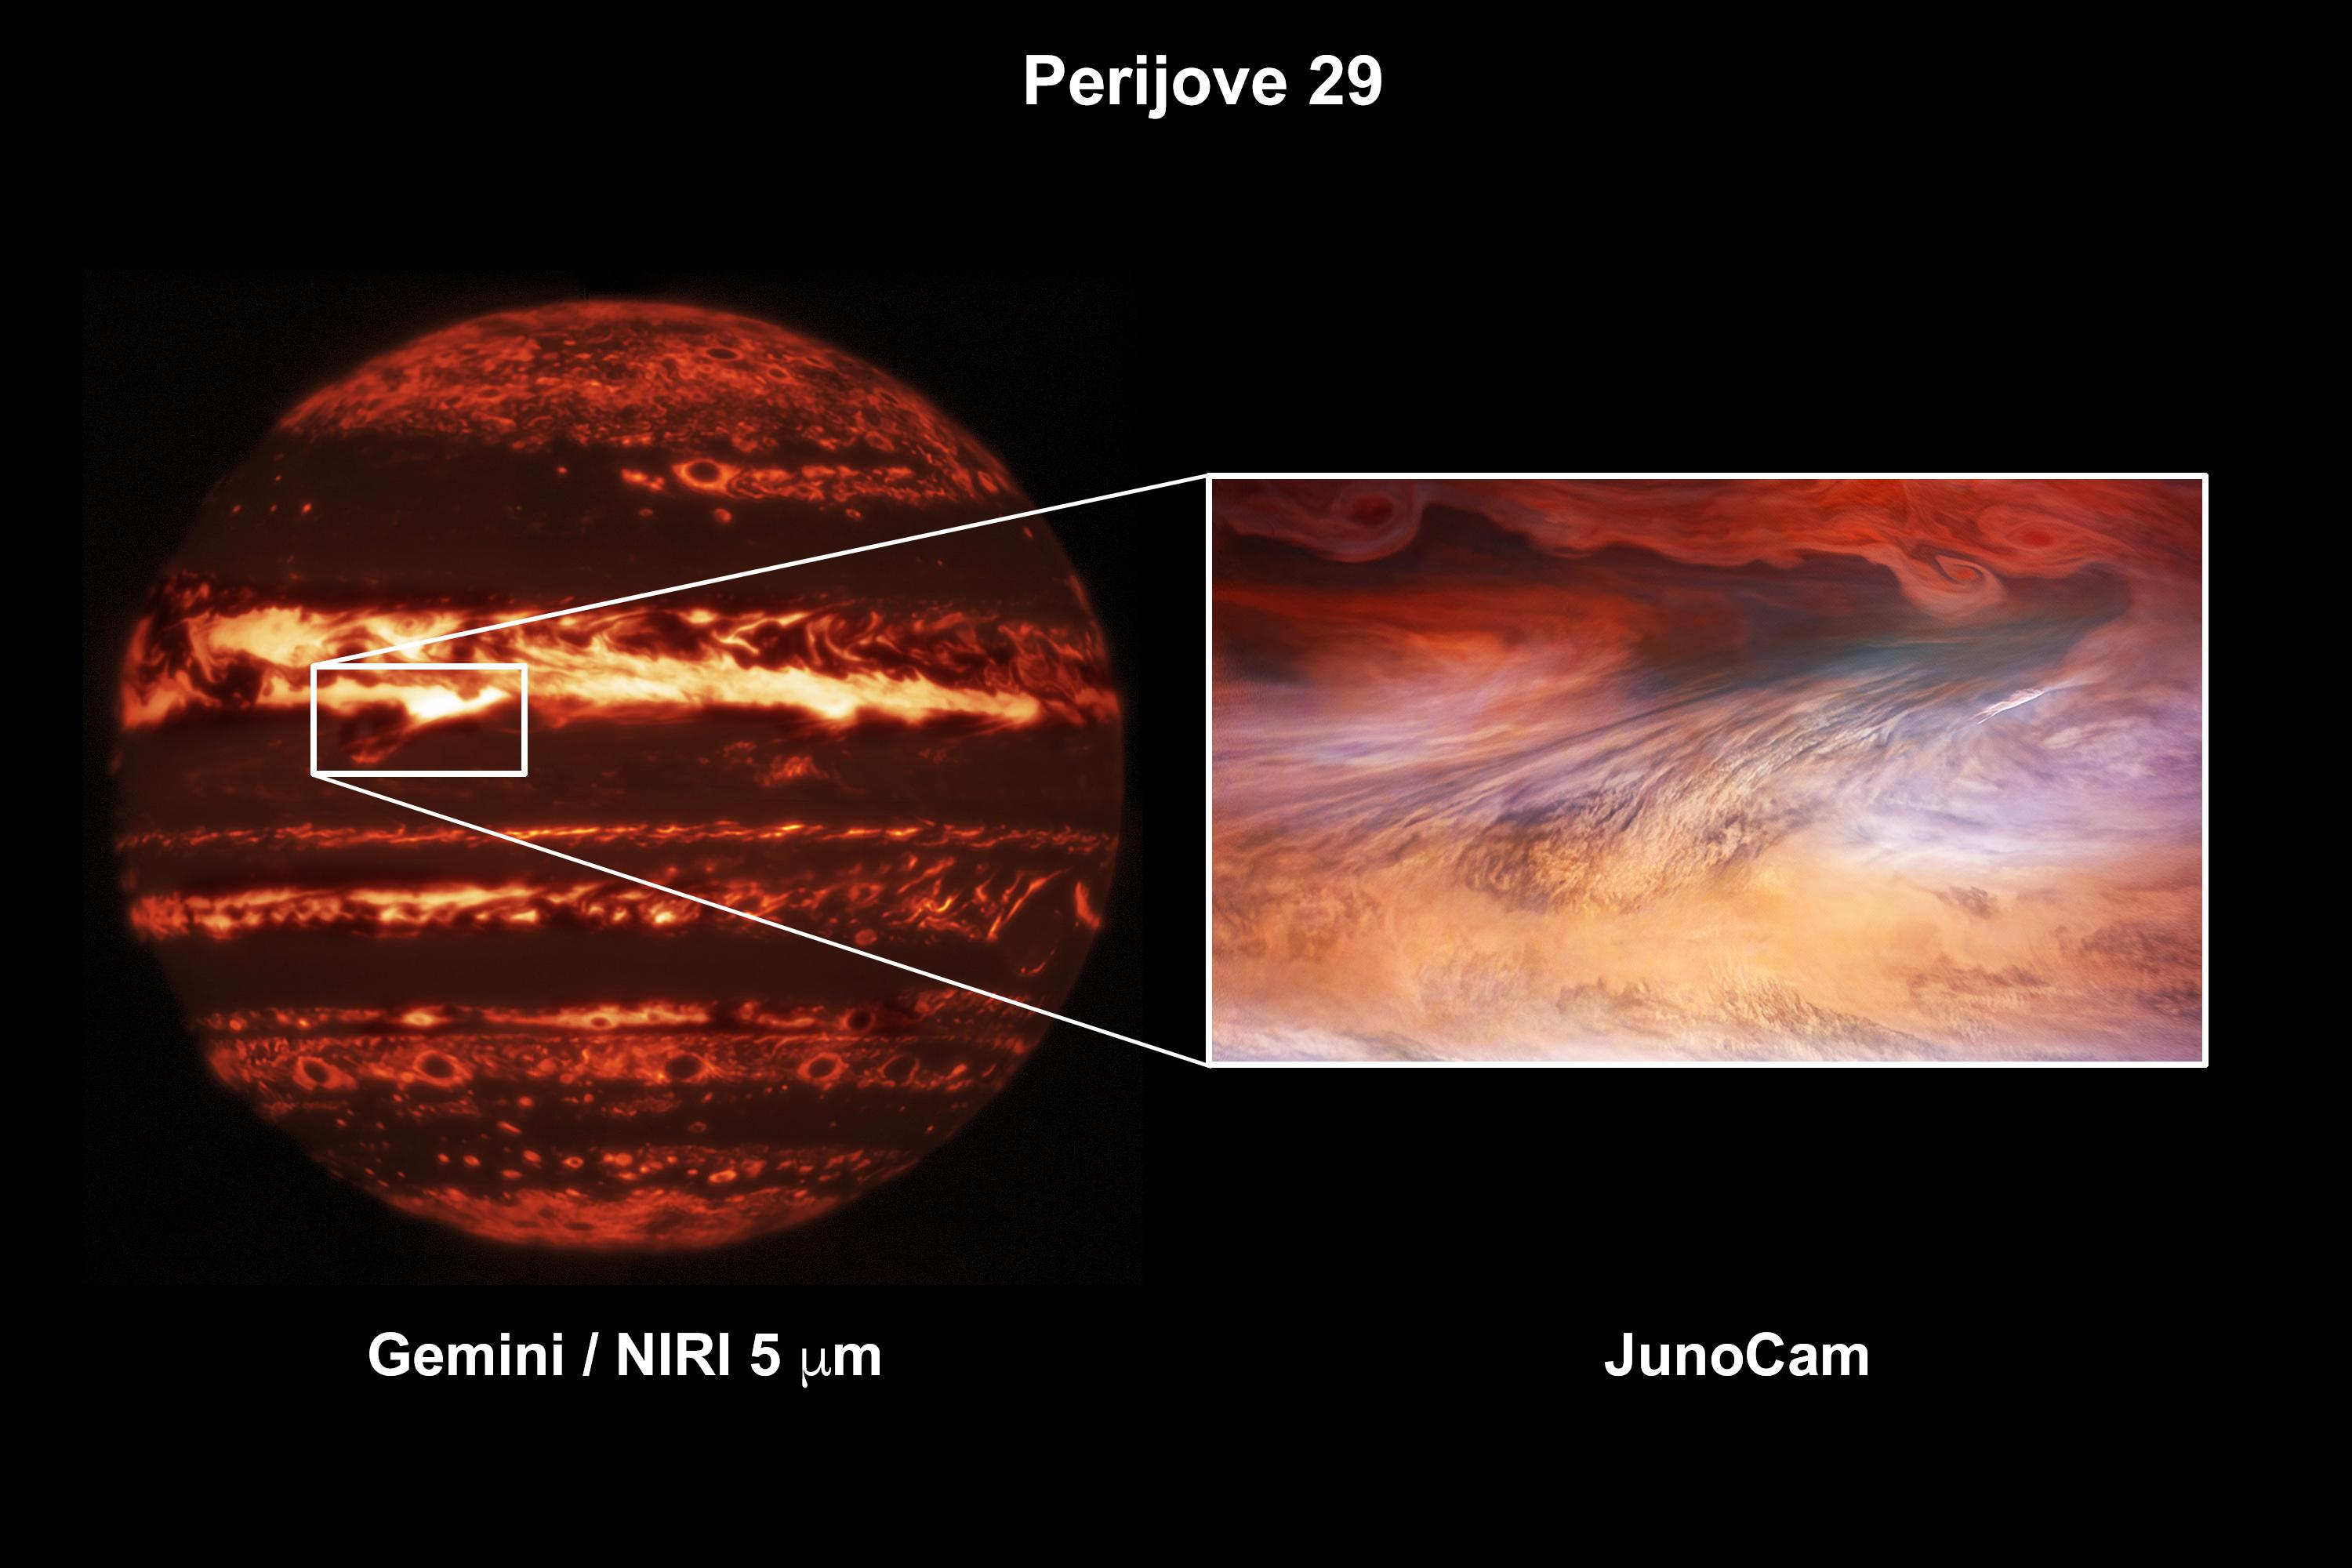
\includegraphics[width=0.9\textwidth]{img/anonimizado.jpg}
			\caption{Imagen inicial anonimizado}
			\label{img: anonimizado src}
		\end{center}
	\end{figure}

	\noindent En mi implementación, he optado por realizar una selección manual de la zona a recortar. Sin embargo, si tuviéramos que procesar muchas imágenes diferentes, la mejor opción sería realizar una máscara binaria, ya que así podríamos aplicarla de manera automática (sin intervención manual del usuario). \\
	
	\noindent El código implementado sería el siguiente:
	
	\begin{lstlisting}[language=Matlab, caption={Implementación anonimizado con \texttt{MATLAB}}]
% 1 - Anonimizado
% Enrique 
% Ref: https://es.mathworks.com/help/images/ref/imcrop.html
clear;

% Cargamos la imagen
img = imread('anonimizado.jpg');


% Representamos la imagen original
figure
imshow(img);
title('Imagen inicial (sin recortar)')

% Recortamos la imagen con un rectangulo
[crop_img, rect_crop] = imcrop(img);

% Manera automatica
%rect_crop = [120 300 2750 1400];    % [xmin ymin width height]
%crop_img = imcrop(img, rect_crop);

% Comparativa imagen original vs imagen recortada
figure
%suptitle('Imagen Anonimizada')

subplot(1,2,1)
imshow(img)
title('Imagen inicial')

subplot(1,2,2)
imshow(crop_img)
title('Imagen recortada utilizando un rectangulo')
	\end{lstlisting}

	\vspace{10px}

	\noindent Una vez ejecutado el código, tendremos como salida una comparativa entre la imagen inicial (ver figura \ref{img: anonimizado src}) y la imagen recortada:
	
	\begin{figure}[h]
		\begin{center}
			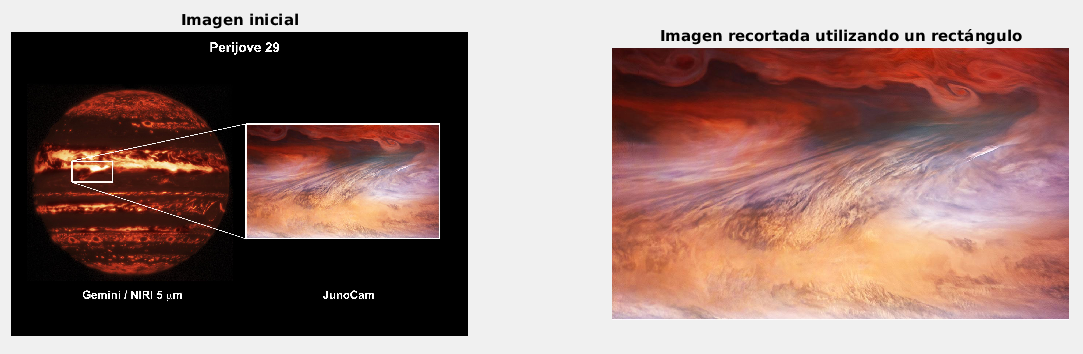
\includegraphics[width=1\textwidth]{img/anonimizado_output.png}
			\caption{Figura de salida al ejecutar script de MATLAB \texttt{anonimizado.m}}
			\label{img: anonimizado output}
		\end{center}
	\end{figure}
	
	\pagebreak
	
	\section{Contraste}
	\noindent En este ejercicio vamos a trabajar las diferentes técnicas que podemos utilizar para mejorar el contraste de una imagen. Para ello vamos a utilizar la siguiente imagen (ver Figura \ref{img: contraste src}).
	
	\begin{figure}[h]
		\begin{center}
			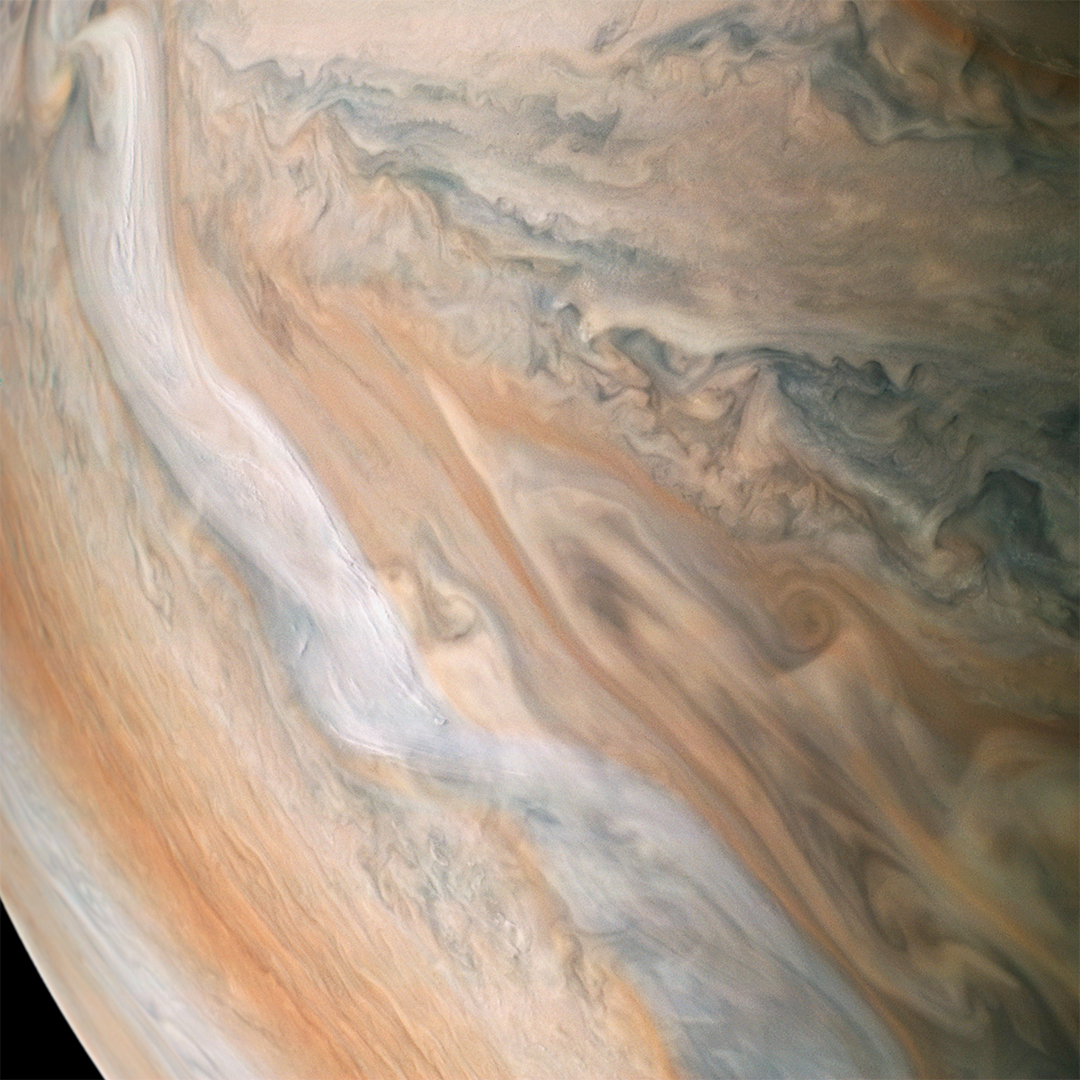
\includegraphics[width=0.5\textwidth]{img/contraste.jpg}
			\caption{Imagen inicial para técnicas de contraste.}
			\label{img: contraste src}
		\end{center}
	\end{figure}

	\noindent Puesto que tenemos diferentes maneras de mejorar el contraste de la imagen, hemos realizado diferentes pruebas con el fin de explorar las posibilidades disponibles. Estas pruebas se resumen en:
	\begin{itemize}
		\item Expansión del histograma, ajuste de iluminación con gamma y filtros espaciales.\\ (\texttt{contraste\_imadjust.m})
		\item Corrección de histograma utilizando herramienta \texttt{imcontrast}.\\
		(\texttt{contraste\_imcontrast.m})
		\item Ajuste canal por canal utilizando \texttt{histeq}.\\
		(\texttt{contrast\_histeq.m})
		\item Ajustes de expansión, \texttt{histeq} y \texttt{adapthiseq} utilizando \texttt{LAB}.\\
		(\texttt{contrast\_shadow.m})
	\end{itemize}

	\noindent Por lo tanto, procedemos a comentar cada una de las diferentes implementaciones.
	
	\pagebreak
	
	\noindent \textbf{\large Expansión del histograma, ajuste de iluminación y filtros espaciales}. \\ 
	
	\noindent En este ejemplo lo que hacemos es aplicar una técnica de expansión del histograma, además de corregir la curva de histograma con el valor \texttt{cte\_gamma}. Por último, intentamos aplicar un filtro espacial (\texttt{prewitt}) para resaltar los cambios de color.
	
	\vspace{10px}
	
	\begin{lstlisting}[language=Matlab, caption={Implementación contraste con expansión de histograma en \texttt{MATLAB}}]
% 2 - Contraste 
% Enrique
% Ref: https://es.mathworks.com/help/images/contrast-enhancement-techniques.html
clear;

% Ajuste del gamma
cte_gamma = 0.95;

% Cargamos la imagen
img = imread('contraste.jpg');
gray_img = rgb2gray(img);
hnorm_org = imhist(gray_img)./numel(gray_img);

% Representamos la imagen original
figure
subplot(2,3,1)
imshow(img);
title('Imagen inicial [RGB]')

subplot(2,3,4)
bar(hnorm_org,'stacked'); 
axis square off, axis([-2 255 0 0.03]), 
title('Histograma original'), 

% Expansion histograma
img_adj = imadjust(img, stretchlim(img), [ ], cte_gamma);
gray_adj = rgb2gray(img_adj);
hnorm_adj = imhist(gray_adj)./numel(gray_adj);

% Representamos la imagen ajustada
subplot(2,3,2)
imshow(img_adj)
title('Imagen expasion histograma')

subplot(2,3,5)
bar(hnorm_adj,'stacked'); 
axis square off, axis([-2 255 0 0.03]), 
title('Histograma ADJ'), 

% Filtro espacial
filter = fspecial('prewitt');
img_filtered = imfilter(img_adj, filter);
img_2 = imadd(img_adj, img_filtered);


gray_filtered = rgb2gray(img_2);
hnorm_filtered = imhist(gray_filtered)./numel(gray_filtered);

% Representamos la imagen filtrada
subplot(2,3,3)
imshow(img_2)
title('Imagen hist expandido + filtro')

subplot(2,3,6)
bar(hnorm_filtered,'stacked'); 
axis square off, axis([-2 255 0 0.03]), 
title('Histograma expandido + filtro'), 
	\end{lstlisting}

	\noindent Una vez ejecutamos dicho código, nos aparece la siguiente figura (ver Figuras \ref{img: contraste imadjust}).
	
	\begin{figure}[h]
		\begin{center}
			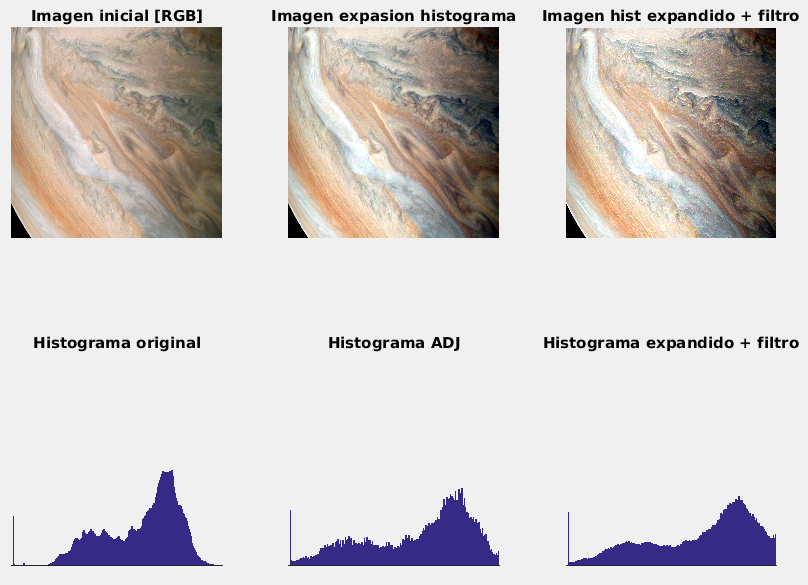
\includegraphics[width=1\textwidth]{img/contrast_imadjust.png}
			\caption{Figura resultante tras ejecución del script \texttt{contrast\_imadjust.m}}
			\label{img: contraste imadjust}
		\end{center}
	\end{figure}
	
	\pagebreak
	
	\noindent \textbf{\large Correción de histograma utilizando herramienta \texttt{imcontrast}}. \\ 
	
	\noindent En este ejemplo lo que hacemos es utilizar la herramienta \texttt{imcontrast} para obtener los valores mínimo y máximo del histograma que creemos que mejora el contraste de nuestra imagen. Para ello, primero ajustamos con dicha herramienta utilizando la imagen en blanco y negro, y luego aplicamos dichos valores en la imagen a color.
	
	\vspace{10px}
	
	\begin{lstlisting}[language=Matlab, caption={Implementación contraste usando \texttt{imcontrast} en \texttt{MATLAB}}]
% 2 - Contraste 
% Enrique
% Ref: https://es.mathworks.com/help/images/contrast-enhancement-techniques.html
clear;

% Cargamos la imagen
img = imread('contraste.jpg');
img = mat2gray(img,[0 255]);
gray_img = rgb2gray(img);
hnorm_org = imhist(gray_img)./numel(gray_img);

figure
imshow(gray_img);
title('Imagen inicial [gris]')
% DESCOMENTAR PARA MOSTRAR HERRAMIENTA
imcontrast;

% Ajustamos con la herramienta imcontrast y sustituimos:
min_hist = 0.2198;
max_hist = 0.8866;
cte_gamma = 0.75;
img_contrast = imadjust(img, [min_hist max_hist], [0 1], cte_gamma);
gray_contrast = rgb2gray(img_contrast);
hnorm_contrast = imhist(gray_contrast)./numel(gray_contrast);

figure,
subplot(2,2,1)
imshow(img, [0 1])
title('Imagen inicial [RGB]')

subplot(2,2,3)
bar(hnorm_org,'stacked'); 
axis square off, axis([-2 255 0 0.03]), 
title('Histograma imagen inicial'), 

subplot(2,2,2)
imshow(img_contrast, [0 1])
title('Imagen ajustada con imcontrast')

subplot(2,2,4)
bar(hnorm_contrast,'stacked'); 
axis square off, axis([-2 255 0 0.03]), 
title('Histograma post ajuste de contraste'),
	\end{lstlisting}

	\pagebreak
	
	\noindent Al ejecutar el script \texttt{contrast\_imcontrast.m}, nos aparecerá la herramienta de \texttt{imcontrast} y diferentes figuras. Deberemos ajustar los valores de la ventana del margen dinámico utilizando dicha herramienta (ver Figura \ref{img: contrast imcontrast 1}), después tendremos que volver a ejecutar el código con esos nuevos valores. De tal manera, nos aparecerá la imagen a color con la corrección de histograma aplicada (ver Figura \ref{img: contrast imcontrast 2}).
	
	\vspace{10px}
	
	\begin{figure}[h]
		\begin{center}
			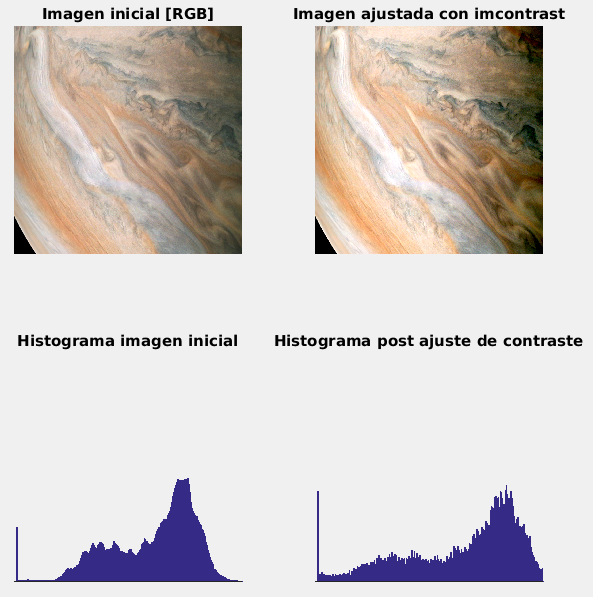
\includegraphics[width=0.8\textwidth]{img/contrast_imcontrast_2.png}
			\caption{Resultado tras ajuste con herramienta \texttt{imcontrast}}
			\label{img: contrast imcontrast 2}
		\end{center}
	\end{figure}
	
	\pagebreak
	
	\begin{figure}[h]
		\begin{center}
			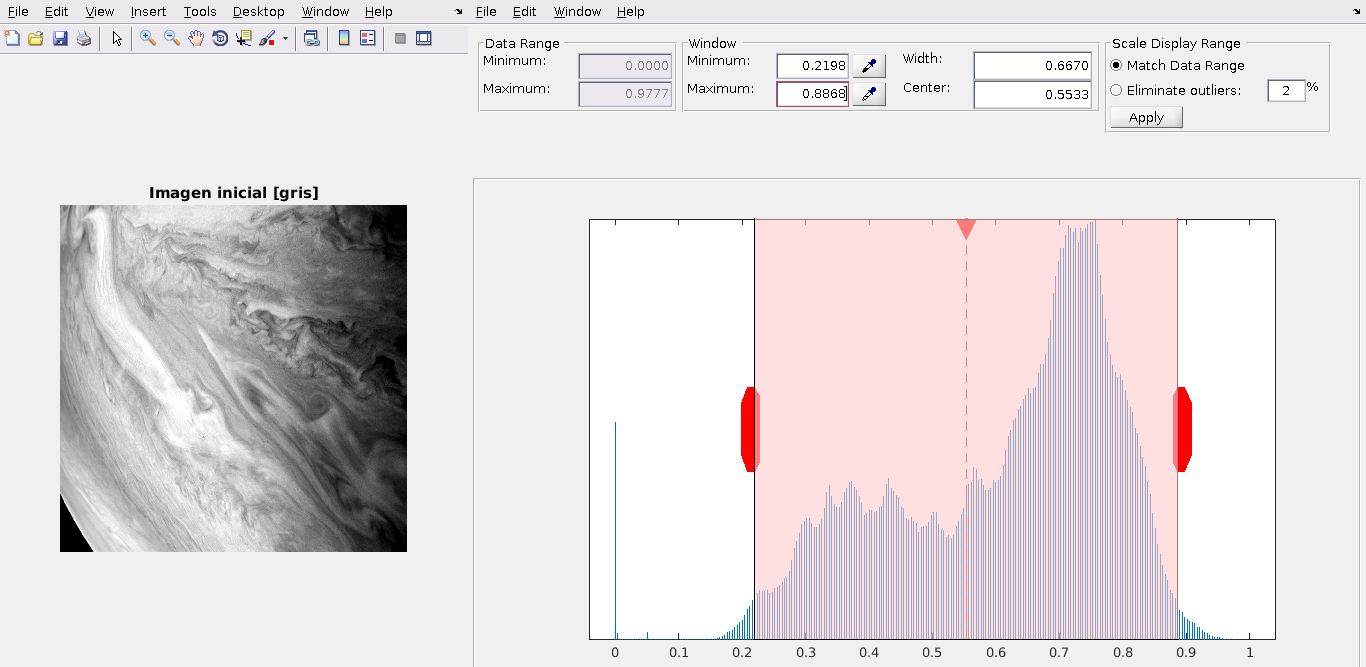
\includegraphics[width=0.85\textwidth]{img/contrast_imcontrast_1.png}
			\caption{Ajuste de histograma utilizando herramienta \texttt{imcontrast}}
			\label{img: contrast imcontrast 1}
		\end{center}
	\end{figure}

	\noindent \textbf{\large Ajuste canal por canal utilizando \texttt{histeq}}. \\ 
	
	\noindent En este ejemplo lo que hacemos es utilizar técnicas de ecualización de histograma. Sin embargo, la función \texttt{histeq} de \texttt{MATLAB} solo admite imágenes con un único canal, por lo que realizamos dicha ecualización por cada canal de color de la imagen. Una vez tenemos cada canal ecualizado, creamos una imagen nueva con la información de esos tres canales.
	
	\begin{lstlisting}[language=Matlab, caption={Implementación contraste utilizando \texttt{histeq} en \texttt{MATLAB}}]
% 2 - Contraste 
% Enrique
% Ref: https://es.mathworks.com/help/images/contrast-enhancement-techniques.html
clear;

% Cargamos la imagen
img = imread('contraste.jpg');
gray_img = rgb2gray(img);
hnorm_org = imhist(gray_img)./numel(gray_img);

figure
subplot(2,2,1)
imshow(img);
title('Imagen inicial')
subplot(2,2,3)
bar(hnorm_org,'stacked'); 
axis square off, axis([-2 255 0 0.03]), 
title('Histograma original'),

% Hacemos histeq a cada canal
R = histeq(img(:,:,1));
G = histeq(img(:,:,2));
B = histeq(img(:,:,3));

% Reconstruimos la imagen
img_contrast(:,:,1) = R;
img_contrast(:,:,2) = G;
img_contrast(:,:,3) = B;

contrast_gray = rgb2gray(img_contrast);
hnorm_gray = imhist(contrast_gray)./numel(contrast_gray);

% Representamos
subplot(2,2,2)
imshow(img_contrast, [])
title('Contraste canal por canal usando histeq')

subplot(2,2,4)
bar(hnorm_gray,'stacked'); 
axis square off, axis([-2 255 0 0.03]), 
title('Histograma post ajuste de contraste'), 
	\end{lstlisting}

	\noindent Una vez ejecutamos el script \texttt{contrast\_histeq.m}, nos aparece una figura con la comparativa entre la imagen original y la imagen ajustada. Como podemos comprobar, si que conseguimos aumentar el contraste, pero los colores de la imagen original se ven modificados (ver Figura \ref{img: contrast histeq}).
	
	\begin{figure}[h!]
		\begin{center}
			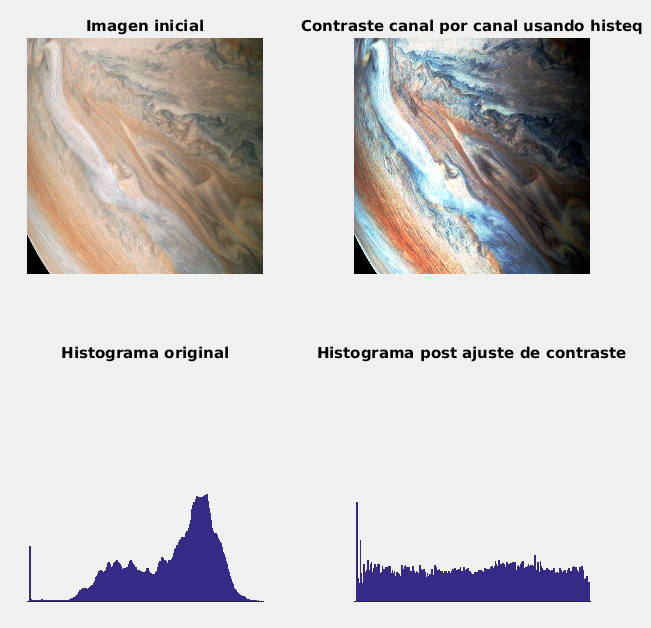
\includegraphics[width=0.65\textwidth]{img/contrast_histeq.png}
			\caption{Figura resultante tras la ejecución del script \texttt{contrast\_histeq.m}}
			\label{img: contrast histeq}
		\end{center}
	\end{figure}

	\noindent \textbf{\large Ajuste de expansión, \texttt{histeq} y \texttt{adapthiseq} utilizando \texttt{LAB}}. \\ 
	
	\noindent En este apartado hemos utilizado técnicas anteriores, pero cambiando a espacio de color tipo \texttt{LAB}, que consiste en un canal para luminancia y dos canales para colores. Hemos comprobado como resultaría utilizar técnicas de expansión de histograma, ecualización de histograma o adaptación de histograma en dicho espacio de color, y posteriormente convertir el resultado a imagen RGB.
	
	\begin{lstlisting}[language=Matlab, caption={Implementanción contraste utilizando \texttt{imadjust}, \texttt{histeq} y \texttt{adapthiseq} en \texttt{LAB}}]
% 2 - Contraste 
% Enrique
% Ref: https://es.mathworks.com/help/images/contrast-enhancement-techniques.html
clear;

% Cargamos la imagen
X = imread('contraste.jpg'); 
shadow_lab = rgb2lab(X);

max_luminosity = 100; 
L = shadow_lab(:,:,1)/max_luminosity;

shadow_imadjust = shadow_lab; 
shadow_imadjust(:,:,1) = imadjust(L)*max_luminosity; 
shadow_imadjust = lab2rgb(shadow_imadjust);
gray_adj = rgb2gray(shadow_imadjust);
hnorm_imadj = imhist(gray_adj)./numel(gray_adj);

shadow_histeq = shadow_lab; 
shadow_histeq(:,:,1) = histeq(L)*max_luminosity; 
shadow_histeq = lab2rgb(shadow_histeq);
gray_histeq = rgb2gray(shadow_histeq);
hnorm_histeq = imhist(gray_histeq)./numel(gray_histeq);

shadow_adapthisteq = shadow_lab; 
shadow_adapthisteq(:,:,1) = adapthisteq(L)*max_luminosity; 
shadow_adapthisteq = lab2rgb(shadow_adapthisteq);
gray_adapt = rgb2gray(shadow_adapthisteq);
hnorm_adapt = imhist(gray_adapt)./numel(gray_adapt);

%% Representamos
figure
subplot(2,3,1)
imshow(shadow_imadjust)
title('Imagen usando imadjust [LAB]')

subplot(2,3,4)
bar(hnorm_imadj,'stacked'); 
axis square off, axis([-2 255 0 0.03]), 
title('Histograma usando imadjust [LAB]'), 

subplot(2,3,2)
imshow(shadow_histeq)
title('Imagen usando histeq [LAB]')

subplot(2,3,5)
bar(hnorm_histeq,'stacked'); 
axis square off, axis([-2 255 0 0.03]), 
title('Histograma usando histeq [LAB]'), 

subplot(2,3,3)
imshow(shadow_adapthisteq)
title('Imagen usando adapthiseq [LAB]')

subplot(2,3,6)
bar(hnorm_adapt,'stacked'); 
axis square off, axis([-2 255 0 0.03]), 
title('Histograma usando adapthiseq [LAB]'), 
	\end{lstlisting}
	
	\vspace{10px}

	\noindent Una vez ejecutamos el script \texttt{contrast\_shadow.m}, nos aparece una figura comparativa entre las tres diferentes técnicas utilizadas.
	
	\begin{figure}[h]
		\begin{center}
			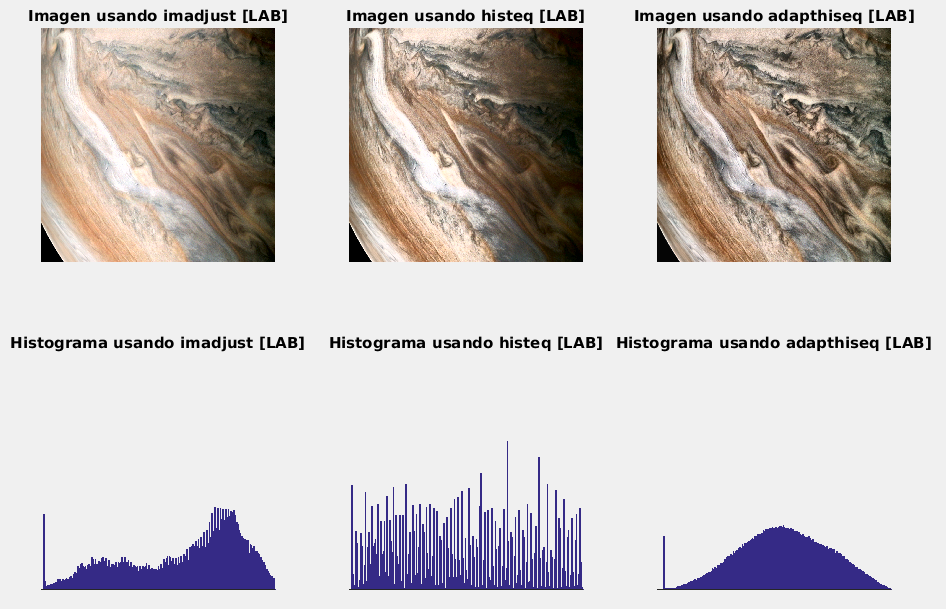
\includegraphics[width=1\textwidth]{img/contrast_shadow.png}
			\caption{Figura resultante tras la ejecución del script \texttt{contrast\_shadow.m}}
			\label{img: contrast shadow}
		\end{center}
	\end{figure}
	
	
	\pagebreak
	
	\section{Iluminación}
	
	\pagebreak
	
	\section{Suavizado}
	
	\noindent En este apartado tenemos que aplicar técnicas de suavizado a la imagen \ref{img: suavizado src}. El objetivo es obtener una imagen en la que se vean suavizados los diferentes desperfectos.
	
	\begin{figure}[h]
		\begin{center}
			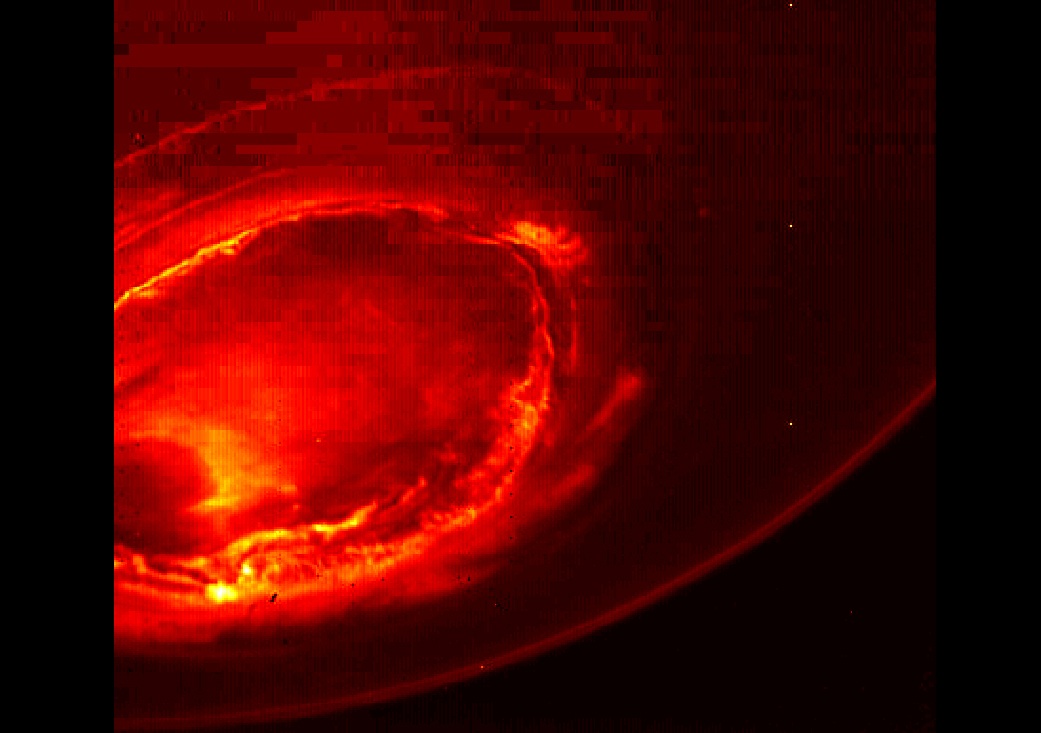
\includegraphics[width=0.8\textwidth]{img/suavizado.jpg}
			\caption{Imagen inicial suavizado}
			\label{img: suavizado src}
		\end{center}
	\end{figure}

	\noindent Para este caso, vamos a utilizar técnicas de filtrado de imagen. Además, vamos a comprar como realizar el filtrado en el dominio del espacio (\texttt{suavizado\_esp.m}) y en el dominio de la frecuencia (\texttt{suavizado\_freq.m}). \\
	
	\noindent \textbf{\large Dominio del espacio} \\
	
	\noindent En el dominio del espacio, vamos a utilizar un filtrado gaussiano, este filtrado lo podríamos implementar con las funciones \texttt{fspecial()} y \texttt{imfilter()}, sin embargo, vamos a utilizar una función especial del paquete de \texttt{Image Processing Toolbox}, llamada \texttt{imgaussfilt()}, que sería equivalente a utilizar las dos funciones (\texttt{fspecial} y \texttt{imfilter}).
	
	\begin{lstlisting}[language=Matlab, caption={Implementación de suavizado en el dominio espacial en \texttt{MATLAB}}]
% 4 - Suavizado
% Enrique
clear;

img_rgb = imread('suavizado.jpg');
cte_gauss = 3;

% Filtramos en el espacio
img_filt = imgaussfilt(img_rgb, cte_gauss,'FilterSize', 19, 'Padding', 'circular');

% Representamos ambas imagenes
figure
subplot(1,2,1),
imshow(img_rgb, []),
axis off image,
title('Imagen original [RGB]')

subplot(1,2,2)
imshow(img_filt, [])
title('Imagen filtrada en el dominio del espacio [RGB]')
	\end{lstlisting}

	\vspace{10px}

	\noindent Como podemos comprobar en la implementación, los parametros del filtro se aplican de manera equivalente a como lo haríamos con las funciones \texttt{fspecial} y \texttt{imfilter}. En este caso, hemos probado con diferentes valores de filtrado para obtener un mejor suavizado. Una vez ejecutamos el script \texttt{suavizado\_esp.m}, obtenemos la siguiente figura comparativa entre la imagen original y la imagen suavizada (ver Figura \ref{img: suavizado esp}).
	
	\vspace{10px}
	
	\begin{figure}[h]
		\begin{center}
			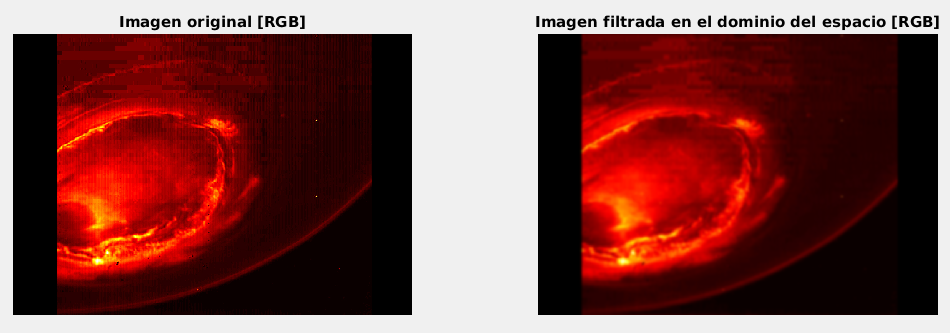
\includegraphics[width=1\textwidth]{img/suavizado_esp.png}
			\caption{Figura resultante al ejecutar el script \texttt{suavizado\_esp.m}}
			\label{img: suavizado esp}
		\end{center}
	\end{figure}

	\pagebreak
	
	\noindent \textbf{\large Dominio de la frecuencia} \\
	
	\noindent En el dominio del espacio también podemos filtrar la imagen, con el objetivo de quitar componentes en frecuencia que nos provoquen esos ``cuadrados'' en el dominio del espacio. Para ello, utilizamos un filtro tipo gaussiano, pero aplicándolo sobre la imagen en frecuencia.
	
	\begin{lstlisting}[language=Matlab, caption={Implementación suavizado en el dominio de la frecuencia en \texttt{MATLAB}}]
% 4 - Suavizado
% Enrique
clear;

img = im2single(imread('suavizado.jpg'));
cte_gauss = 4.5;

% Representamos imagen original
figure,
subplot(1,2,1)
imshow(img),
title('Imagen original [RGB]')

% Aplicamos filtro gaussiano sobre las dimensiones de la imagen (733 1041)
filter = fspecial('gaussian', [733 1041], cte_gauss);

% Canal R
F1 = fftshift(fft2(img(:,:,1)));
mask1 = fftshift(psf2otf(filter,[size(img(:,:,1), 1), size(img(:,:,1), 2)]));

% Canal G
F2 = fftshift(fft2(img(:,:,2)));
mask2 = fftshift(psf2otf(filter,[size(img(:,:,3), 1), size(img(:,:,3), 2)]));

% Canal B
F3 = fftshift(fft2(img(:,:,3)));
mask3 = fftshift(psf2otf(filter,[size(img(:,:,3), 1), size(img(:,:,3), 2)]));

% Reconstruimos la imagen a color
filtered_img(:,:,1) = ifft2(ifftshift(F1 .* mask1));
filtered_img(:,:,2) = ifft2(ifftshift(F2 .* mask2));
filtered_img(:,:,3) = ifft2(ifftshift(F3 .* mask3));

% Representamos en el dominio de la frecuencia
%F = fft2(img_rgb(:, :, 2));
%S = fftshift(log(1+abs(F)));
%figure
%imshow(S, []),
%title('Representacion del espectro (log)');

% Representamos la imagen suavizada
subplot(1,2,2)
imshow(abs(filtered_img)),
axis off image,
title('Imagen filtrada en el dominio de la frecuencia [RGB]')
	\end{lstlisting}
	
	\pagebreak
	
	\noindent Para este caso, lo que hacemos es aplicar un filtro a la imagen en frecuencia. Como el filtro solo nos permite aplicarlo sobre un canal a la vez, descomponemos la imagen en los canales R, G y B, para aplicar el filtro y posteriormente reconstruir la imagen. Una vez ejecutamos el script \texttt{suavizado\_freq.m}, nos aparece una figura comparativa entre la imagen inicial y la imagen suavizada en frecuencia (ver Figura \ref{img: suavizado freq}).
	
	\begin{figure}[h]
		\begin{center}
			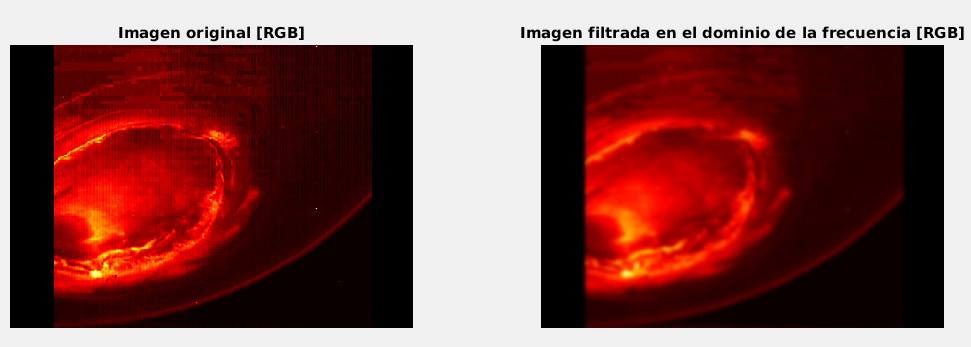
\includegraphics[width=1\textwidth]{img/suavizado_freq.png}
			\caption{Figura resultante al ejecutar el script \texttt{suavizado\_freq.m}}
			\label{img: suavizado freq}
		\end{center}
	\end{figure}
	
	\pagebreak
	
	\section{Realzado}
	
	\noindent En este ejercicio tenemos que aplicar técnicas de realzado para obtener más detalles en la imagen X. Para ello, aplicaremos diferentes filtros, con el objetivo de resaltar los cambios entre las diferentes zonas de color de la imagen.
	
	\begin{figure}[h]
		\begin{center}
			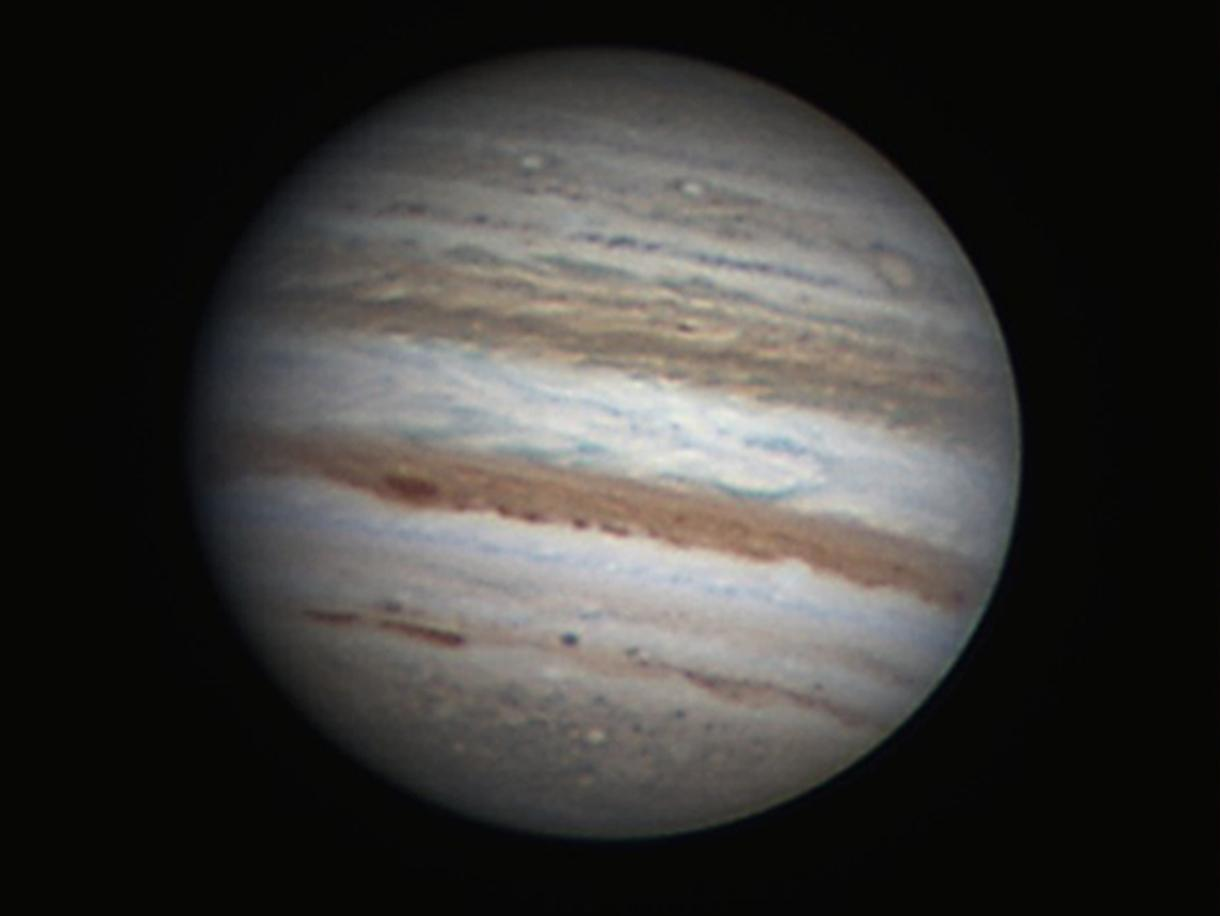
\includegraphics[width=0.7\textwidth]{img/realzado.jpg}
			\caption{Imagen inicial realzado}
			\label{img: realzado src}
		\end{center}
	\end{figure}

	\noindent Para realzar la imagen podemos aplicar filtros directamente sobre la imagen original. En este caso, hemos aplicado un preajuste del histograma, para hacer que el margen dinámico ocupe todo el histograma. Una vez tenemos la imagen preajustada, la filtramos con \texttt{prewitt} o \texttt{sobel}.
	
	\begin{lstlisting}[language=Matlab, caption={Implementación de filtros para el realzado en \texttt{MATLAB}}]
% 5 - Realzado
% Enrique
clear;

img_rgb = imread('realzado.jpg');

% Preajuste expansion margen dinamico
img_adj = imadjust(img_rgb, stretchlim(img_rgb), [ ]);

% Caso uno, prewitt
filter = fspecial('prewitt');
img_filtered = imfilter(img_adj, filter, 'replicate');
%img_rgb_1 = imadd(img_adj, img_filtered);
img_rgb_1 = img_adj - img_filtered;

% Caso dos, sobel
filter = fspecial('sobel');
img_filtered = imfilter(img_adj, filter, 'replicate');
%img_rgb_2 = imadd(img_adj, img_filtered);
img_rgb_2 = img_adj - img_filtered;

figure
subplot(2,2,1)
imshow(img_rgb, [])
title('Imagen original')

subplot(2,2,2)
imshow(img_adj, [])
title('Imagen preadjustada')

subplot(2,2,3)
imshow(img_rgb_1, [])
title('Imagen realzada (prewitt)')

subplot(2,2,4)
imshow(img_rgb_2, [])
title('Imagen realzada (sobel)')

	\end{lstlisting}

	%\vspace{10px};
	\pagebreak
	
	\noindent Una vez ejecutado el código, obtenemos como salida una figura comparativa entre la imagen original, la imagen preajustada y las opciones de filtrado (\texttt{prewitt} y \texttt{sobel}).
	
	\begin{figure}[h]
		\begin{center}
			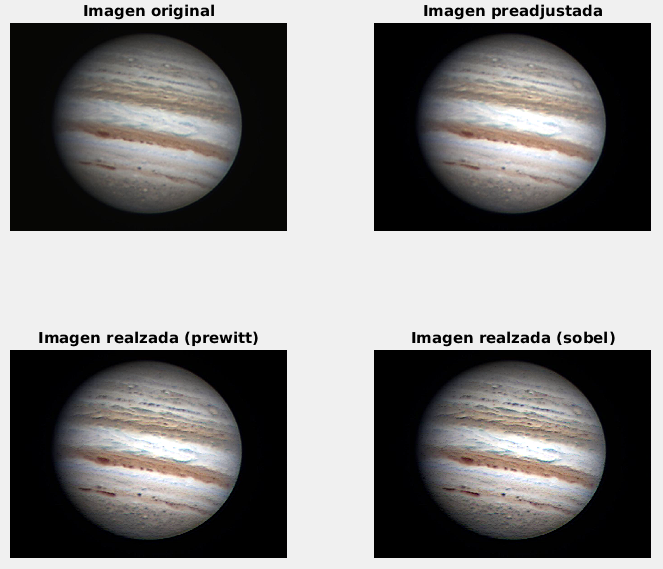
\includegraphics[width=0.9\textwidth]{img/realzado_output.png}
			\caption{Imagen inicial ruido}
			\label{img: realzado output}
		\end{center}
	\end{figure}

	\noindent Si tuvieramos que quedarnos con uno de los filtrados, el filtro \texttt{sobel} parece que realza mucho más las transiciones de color, cosa que en el caso de \texttt{prewitt} también distinguimos, pero en esta imagen en concreto el realzado es menor que respecto a \texttt{sobel}.
	
	\pagebreak
	
	\section{Ruido}
	
	\noindent En este ejercicio tenemos que aplicar técnicas de reducción de ruido a la imagen \ref{img: ruido src}. Lo primero que tendríamos que intentar hacer es ver que tipo de ruido es, en este caso creemos que es ruido tipo ``sal y pimienta''.
	
	\begin{figure}[h]
		\begin{center}
			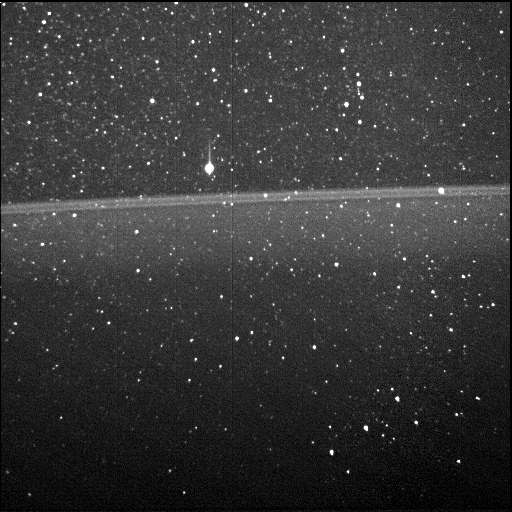
\includegraphics[width=0.7\textwidth]{img/ruido.jpg}
			\caption{Imagen inicial ruido}
			\label{img: ruido src}
		\end{center}
	\end{figure}
	
	\noindent Puesto que el ruido de la imagen se puede entender como un ruido de tipo ``sal y pimienta'', una de las técnicas que podemos utilizar es ejecutar de manera recursiva un filtro de mediana sobre la imagen.
	
	\begin{lstlisting}[language=Matlab, caption={Implementación filtro mediana para reducir ruido en \texttt{MATLAB}}]
% 6 - Ruido Sal y Pimienta
% Enrique
clear;

img_rgb = 'ruido.jpg';
neighborn = 4;
times = 5;

img = imread(img_rgb);
img = mat2gray(img,[0 255]);
img = rgb2gray(img);

figure
subplot(1,2,1)
imshow(img, [])
title('Imagen original [RGB]')

% Aplicamos filtro mediana
img_median = img;
for n=1:times,
img_median = medfilt2(img_median, [1 1]*neighborn);
end

% Representamos resultado
subplot(1,2,2)
imshow(img_median, []),
axis off image,
title(['Imagen eliminado el ruido usando filtro mediana con N=' num2str(neighborn) ' T=' num2str(times) ])
	\end{lstlisting}

	\vspace{10px}

	\noindent Una vez ejecutado el código, tendremos como salida una comparativa entre la imagen inicial (ver figura \ref{img: ruido src}) y imagen resultante tras eliminar el ruido ``sal y pimienta'':
	
	\begin{figure}[h]
		\begin{center}
			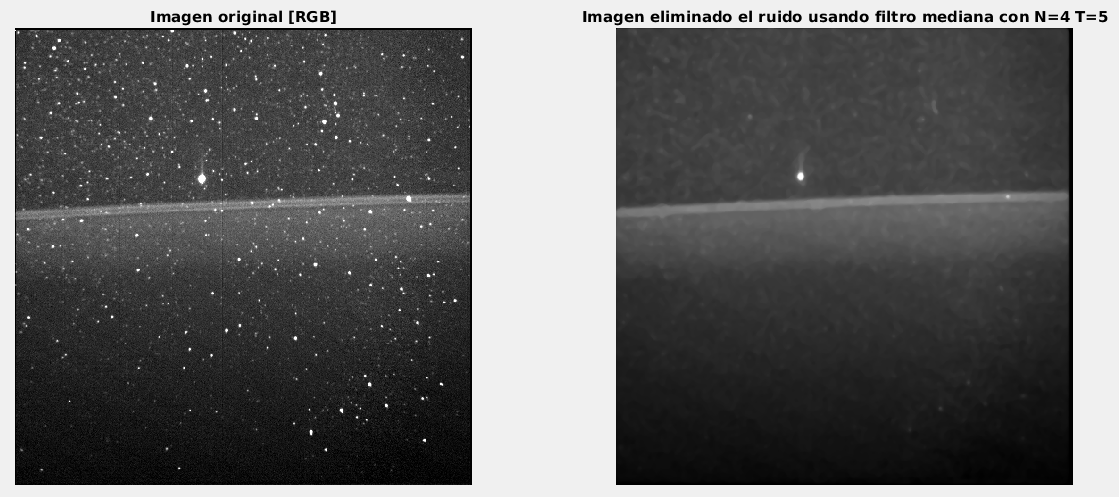
\includegraphics[width=1\textwidth]{img/ruido_output.png}
			\caption{Figura de salida al ejecutar script de MATLAB \texttt{ruido.m}}
			\label{img: ruido output}
		\end{center}
	\end{figure}
	
	\pagebreak
	
	\section{Patrones}
	\noindent En este ejercicio vamos a practicar la técnica de detección de patrones utilizando el coeficiente de correlación de Pearson. Para ello, trabajamos sobre la imagen \ref{img: patrones src}.
	
	\begin{figure}[h]
		\begin{center}
			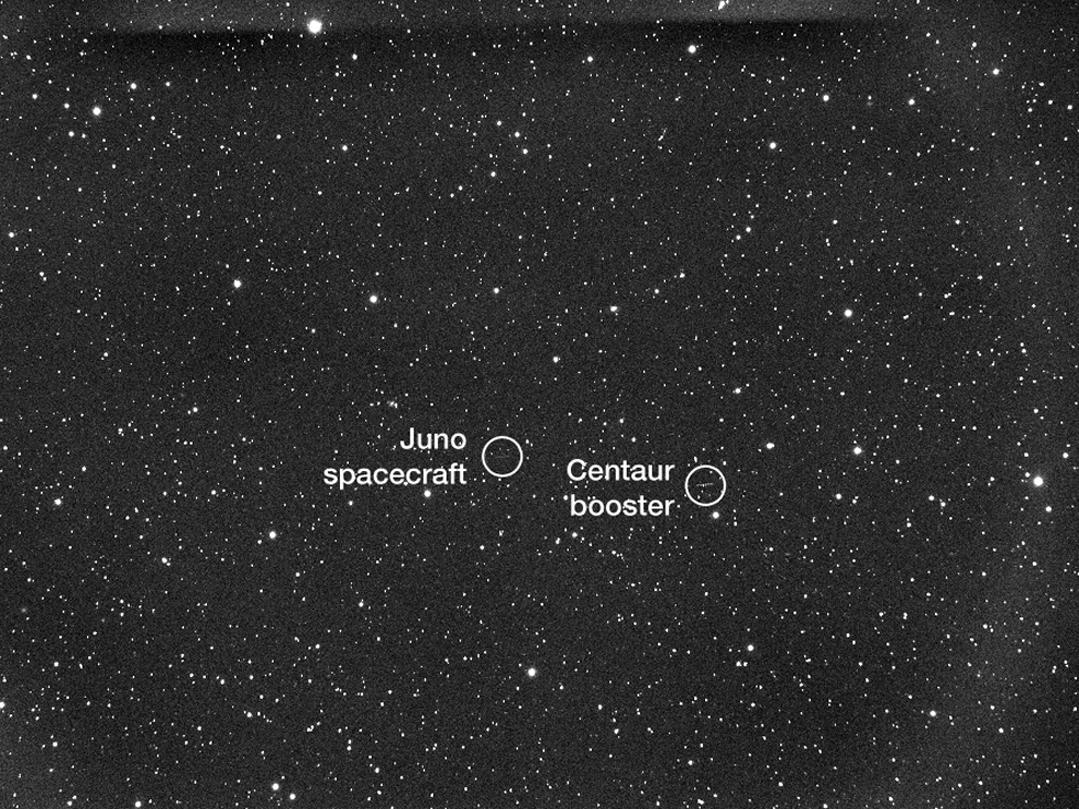
\includegraphics[width=0.8\textwidth]{img/patrones.jpg}
			\caption{Imagen inicial de patrones}
			\label{img: patrones src}
		\end{center}
	\end{figure}

	\noindent Utilizando la imagen \ref{img: patrones src}, elegimos un patrón (una estrella) que queramos encontrar coincidencias. Una vez encontradas las coincidencias sobre el patrón establecido, volvemos a representar la imagen original resaltando dichas coincidencias.
	
	\begin{lstlisting}[language=Matlab, caption={Implementación detección de patrones en \texttt{MATLAB}}]
% 7 - Patrones
% Enrique
% ref: https://es.mathworks.com/matlabcentral/answers/90094-how-to-convolved-two-image
clear;

img_rgb = 'patrones.jpg';
threshold_corre = 0.55;
threshold_stars = 0.85;

img_rgb = single(imread(img_rgb));
img_rgb = mat2gray(img_rgb,[0 255]);
img = rgb2gray(img_rgb);

% Funciones en una linea
lambda_covar = @(A,B) conv2(A-mean(A(:)), B(end:-1:1,end:-1:1)-mean(B(:)), 'valid');
lambda_autocovar = @(A,B) conv2(A.*A, ones(size(B)), 'valid')-conv2(A, ones(size(B)), 'valid').^2/numel(B);

% Imagen original
figure,
imshow(img, [0 1]), 
axis off image,
title('Imagen original [RGB]')

% Ejemplo de pattern: Pattern = PatternDetection(163:178,84:100);
p_img = round(ginput(2));       % Warning, must be integer to use as index
selected_pattern = img(p_img(1,2):p_img(2,2), p_img(1,1):p_img(2,1));

% Imagen del pattern seleccionado
figure,
subplot(1,2,1), 
imshow(selected_pattern, [0 1]), 
axis off image,
title('Patron seleccionado')

subplot(1,2,2), 
mesh(selected_pattern), 
axis off square, 
set(gca,'XDir','reverse'), 
title('Patron seleccionado (plot en elevacion)')


%% Deteccion del patron
coef_pearson = lambda_covar(single(img), single(selected_pattern));
coef_pearson_dem = sqrt(lambda_autocovar(img, selected_pattern).*lambda_autocovar(selected_pattern, selected_pattern));
index = find(coef_pearson_dem ~= 0);
coef_pearson(index) = coef_pearson(index)./coef_pearson_dem(index);

coef_pearson = padarray(coef_pearson, floor((size(selected_pattern)-1)/2), 0, 'post');
coef_pearson = padarray(coef_pearson, ceil((size(selected_pattern)-1)/2), 0, 'pre');
coef_pearson = coef_pearson.*(coef_pearson > threshold_corre);

figure,
subplot(1,2,1), 
imshow(coef_pearson*50+img, [0 1]),
axis off image, 
title('Patrones detectados resaltados en amarillo')
% Resaltamos las ocurrencias con amarillo
map=colormap('gray'); 
map(256,:)=[1 1 0]; colormap(map)


subplot(1,2,2), 
mesh(coef_pearson), 
axis square, 
set(gca,'YDir','reverse'), 
title('Ocurrencias de la deteccion del patron (plot en elevacion)')

% Display number of ocurrencies on coef pearson
number_stars = sum(sum(coef_pearson > threshold_stars));
disp(['Numero de estrellas detectadas: ' num2str(number_stars)]);
	\end{lstlisting}

	\vspace{20px}

	\noindent Una vez ejecutamos el código, primero nos aparece una figura con título ``\textit{Imagen original [RGB]}'', en la que tendremos que seleccionar la estrella a detectar (ver Figura \ref{img: patrones 1}). Tendremos que hacer click en las diagonales superior izquierda e inferior derecha del patrón (estrella) que queramos detectar, nos aparecerá una figura con el patrón que hemos seleccionado (ver Figura \ref{img: patrones 2})
	
	\vspace{20px}
	
	\begin{figure}[h]
		\begin{center}
			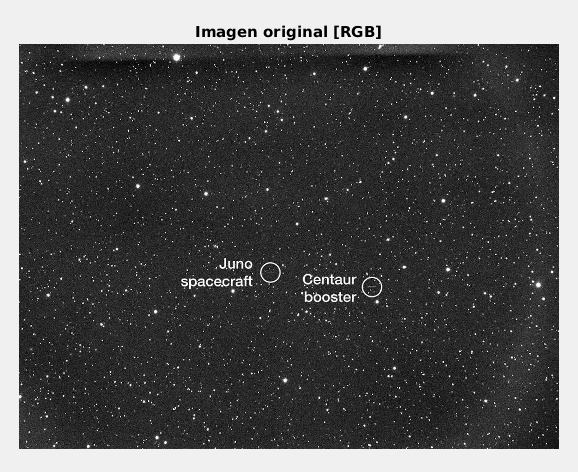
\includegraphics[width=0.75\textwidth]{img/patrones_1.png}
			\caption{Imagen para seleccionar el patrón a buscar}
			\label{img: patrones 1}
		\end{center}
	\end{figure}
	
	\pagebreak
	
	\begin{figure}[h]
		\begin{center}
			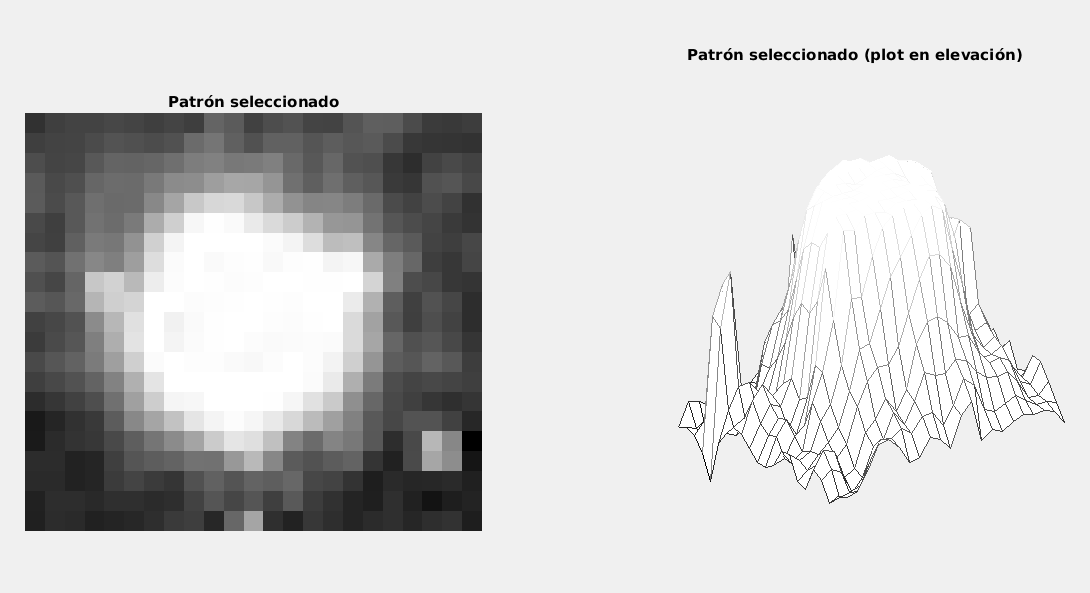
\includegraphics[width=0.8\textwidth]{img/patrones_2.png}
			\caption{Figura resultante una vez seleccionamos el patrón}
			\label{img: patrones 2}
		\end{center}
	\end{figure}

	\noindent Una vez seleccionamos el patrón, podemos comprobar que además de la figura de la imagen \ref{img: patrones 2}, nos aparecer otra figura en la que se nos resalta en color amarillo las ocurrencias que tenemos en la imagen, en comparación con nuestro patrón (ver Figura \ref{img: patrones 3}). 
	
	\begin{figure}[h!]
		\begin{center}
			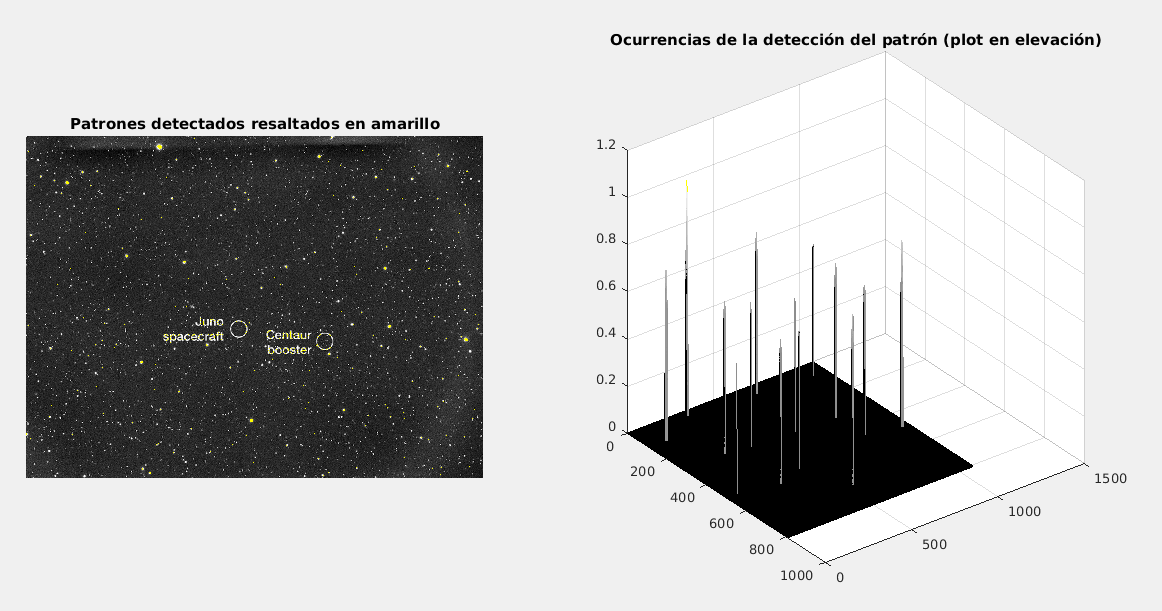
\includegraphics[width=1\textwidth]{img/patrones_3.png}
			\caption{Figura resultante una vez seleccionamos el patrón}
			\label{img: patrones 3}
		\end{center}
	\end{figure}

	\pagebreak
	
	\noindent Además, hemos cuantificado el número de estrellas detectadas. Para ello, hemos tenido en cuenta un valor umbral por el cual consideramos una ocurrencia como una estrella. En la consola de MATLAB podemos comprobar cuantas estrellas hemos detectado (ver Figura \ref{img: patrones 4}).

	\begin{figure}[h]
		\begin{center}
			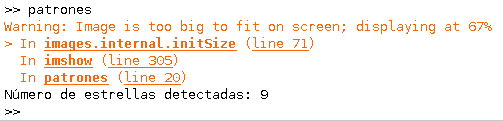
\includegraphics[width=0.9\textwidth]{img/patrones_4.png}
			\caption{Número de estrellas detectadas, mensaje en la consola en MATLAB }
			\label{img: patrones 4}
		\end{center}
	\end{figure}
	
	\pagebreak
	
	\section{Pseudocoloración}
	
	\noindent En este ejercicio tenemos que aplicar técnicas de pseudocoloración a la imagen de un planeta (ver Figura X), con esto pretendemos ver detalles, que en el caso de ver la imagen en niveles de gris no veríamos.
	
	\begin{figure}[h]
		\begin{center}
			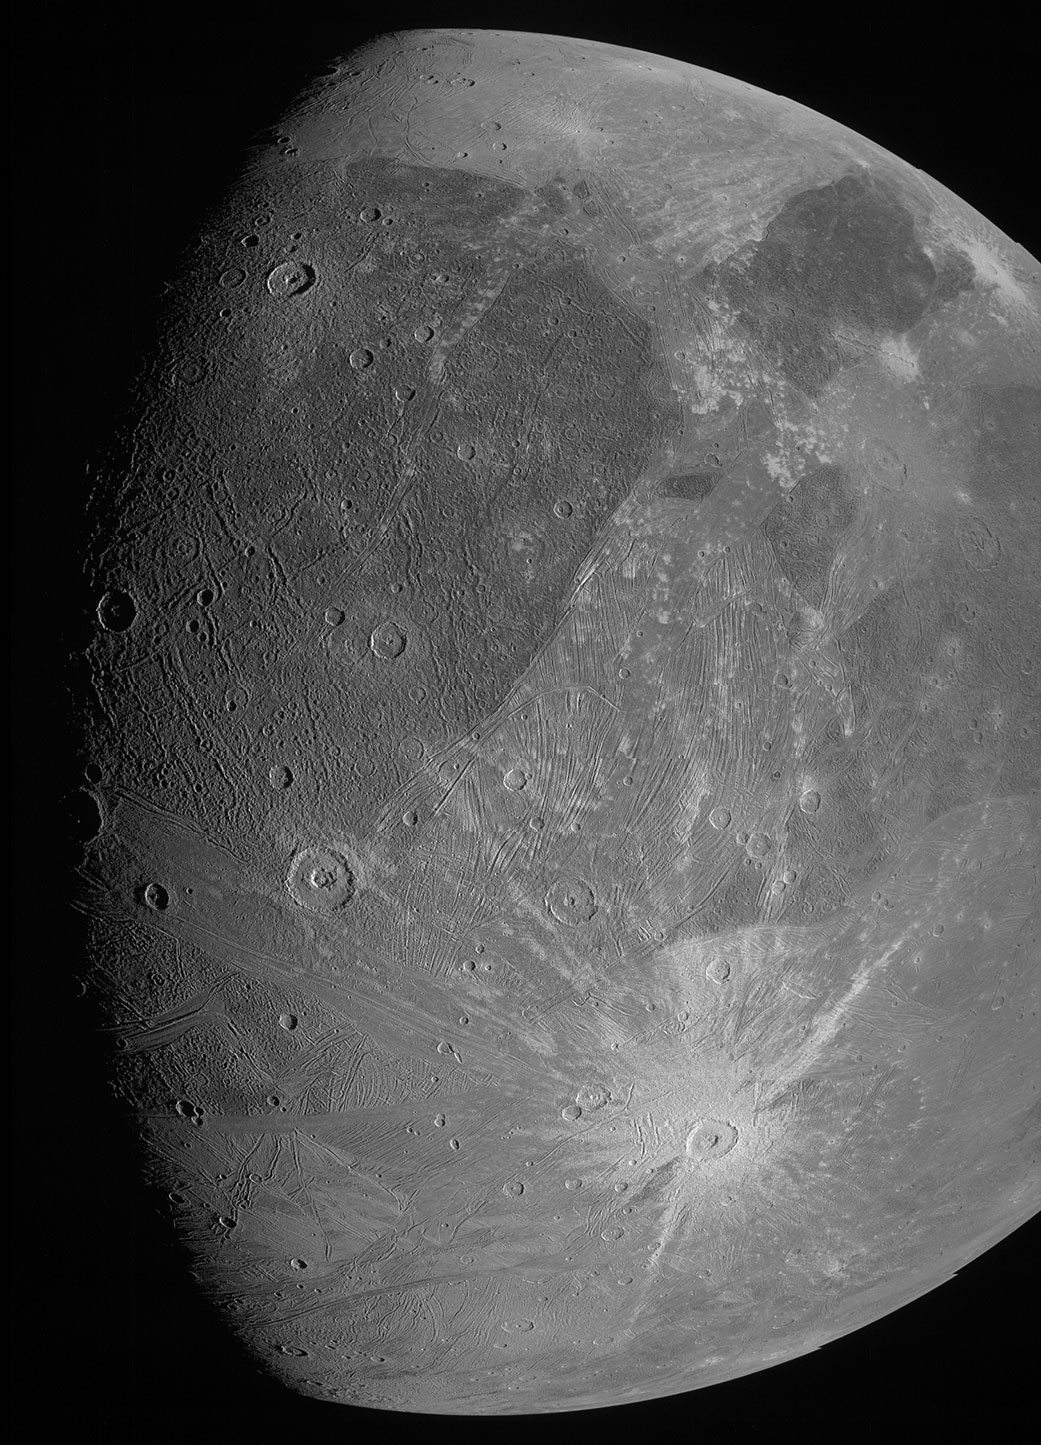
\includegraphics[width=0.4\textwidth]{img/pseudocoloracion.jpg}
			\caption{Imagen inicial pseudocoloración}
			\label{img: pseudocoloración src}
		\end{center}
	\end{figure}

	\noindent Para la resolución de este ejercicio hemos usado la técnica de coloración de una imagen dependiendo de su nivel de gris. Para ello, hemos probado todos los mapas de colores que MATLAB nos ofrece, sin embargo solo \texttt{copper}, \texttt{pink}, \texttt{bone}, \texttt{hot} y \texttt{parula} nos aportaban resultados útiles.
	
	\begin{lstlisting}[language=Matlab, caption={Implementación de pseucoloración en \texttt{MATLAB}}]
		% 8 - Pseudocoloracion por nivel de gris
		% Enrique 
		
		img_rgb = 'pseudocoloracion.jpg';
		gray_lvl = 64;
		
		img = imread(img_rgb);
		img = mat2gray(img,[0 255]);
		img = rgb2gray(img);
		
		% Utilizamos 64 niveles de gris
		img_colored = grayslice(img, gray_lvl);
		
		
		% Representamos cada una de las coloraciones
		figure
		subplot(2,3,1),
		subimage(img);
		axis off image,
		title('Imagen original en escala de gris')
		
		subplot(2,3,2),
		subimage(img_colored, copper(gray_lvl));
		axis off image,
		title('Pseudocoloracion (copper)')
		
		subplot(2,3,3),
		subimage(img_colored, pink(gray_lvl));
		axis off image,
		title('Pseudocoloracion (pink)')
		
		subplot(2,3,4),
		subimage(img_colored, bone(gray_lvl));
		axis off image,
		title('Pseudocoloracion (bone)')
		
		subplot(2,3,5),
		subimage(img_colored, hot(gray_lvl));
		axis off image,
		title('Pseudocoloracion (hot)')
		
		subplot(2,3,6),
		subimage(img_colored, parula(gray_lvl));
		axis off image,
		title('Pseudocoloracion (parula)')
	\end{lstlisting}
	
	%\vspace{10px}
	\pagebreak
	
	\noindent Una vez ejecutado el código, tendremos como salida una comparativa entre la imagen inicial (ver figura \ref{img: pseudocoloración src}) y las diferentes imágenes resultantes tras aplicar pseudocoloración:
	
	\begin{figure}[h]
		\begin{center}
			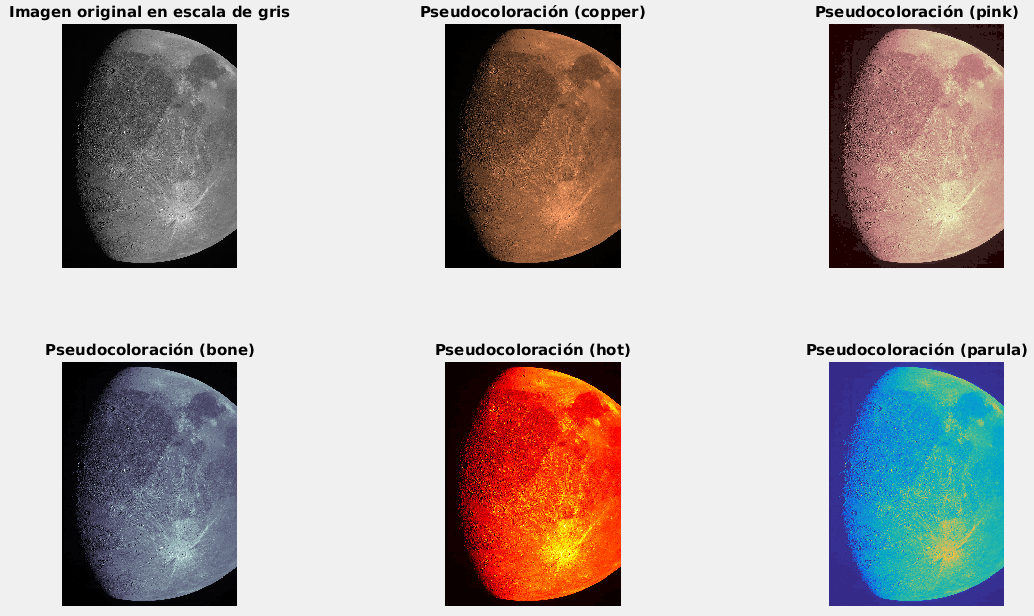
\includegraphics[width=1\textwidth]{img/pseudocoloracion_output.png}
			\caption{Figura de salida al ejecutar script de MATLAB \texttt{pseudocoloracion.m}}
			\label{img: pseudocoloracion output}
		\end{center}
	\end{figure}

	\noindent Si tuviera que elegir entre alguna de las imágenes obtenidas, considero que con \texttt{hot} y \texttt{parula} podemos distinguir más detalles, sin embargo el resto de coloraciones también aportan más detalle que la original.
	
	\pagebreak
\end{document}